\chapter{Set up Droid@Screen}
\label{ch:droid_setup}
\section{Environmental setup}
There is a detail guideline from Droid@Screen official page \cite{droid_setup}. Here I give you another way to configure the application with less effort.

\subsection{Install Java}
Droid@Screen is a Java program, so you need to have Java installed. Get the Java installer from Oracle and go for Java version 7 or later.

\subsection{Install and configure Android \acrshort{sdk}}
Download and install the Android \acrfull{sdk}. You can choose the one with or without IDE depending on your need for building Android application or not.
\newline
After successful installation, open SDK Manager and install Android SDK platform-tools
    
    \begin{figure}[H]
		\centering
		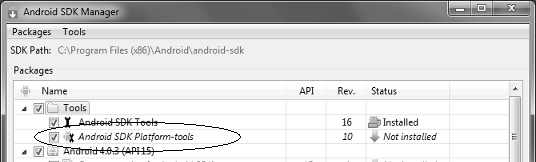
\includegraphics[scale=0.75]{Chapters/Fig/sdk_mng.png}
		\caption{Select SDK platform-tools}
		\label{fig:sdk_mng}
	\end{figure}

\subsection{Configure your Android device}
Enable USB debugging on your device. Then plug in the \acrshort{usb} cable between your device and \acrshort{pc}.
    
    \begin{figure}[H]
		\centering
		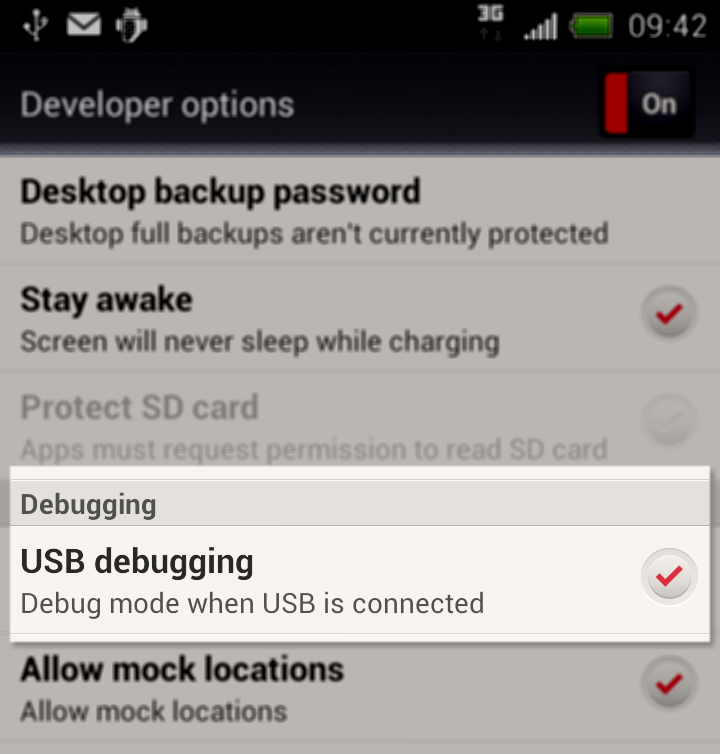
\includegraphics[scale=0.5]{Chapters/Fig/usb-db.png}
		\caption{Enable USB debugging}
		\label{fig:usb-db}
	\end{figure}
	
Install the USB drivers for your phone/tablet. You can obtain appropriate driver from device's vendor or via Windows update (Windows 8 or above).

\subsection{Download and install the latest version of Droid@Screen}
Go to the download page to get Droid@Screen for your computer at \url{http://droid-at-screen.org/download.html}.
\newline
If you prefer the second approach in Appendix \ref{ch:img_capture}, my modified version is available here:  \url{https://github.com/alfrededison/thesis-report/blob/2f0cc6d53dab41e691ec0be2bdf3946f8fdb57cb/Appendices/droidAtScreen-1.2.jar}

\subsection{Launch Droid@Screen}
On Windows, if you install Java properly, just double click on downloaded file.
\newline
For the first time, it will prompt you for the path of ADB. Just navigate to the installation directory of the Android SDK and then into platform-tools/. You should there see the adb.exe file (on Windows).

    \begin{figure}[H]
		\centering
		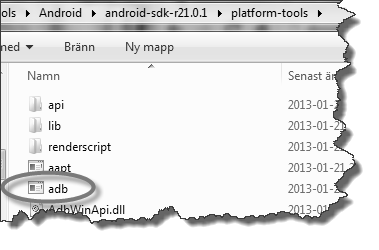
\includegraphics[scale=0.75]{Chapters/Fig/adb.png}
		\caption{ADB location}
		\label{fig:adb}
	\end{figure}
    
\section{Capture screen to image}
If you choose first approach, which is screen capture, you should simply region the displayed mobile screen. Nonetheless, second approach demands one more step in preparation.

When mobile screen is already displayed on the application, click on Recording icon.

	\begin{figure}[H]
		\centering
		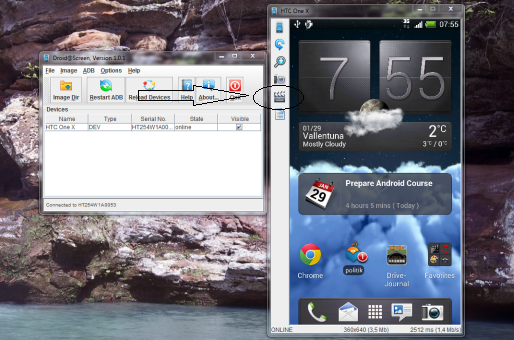
\includegraphics[scale=0.75]{Chapters/Fig/record.png}
		\caption{Target record icon}
		\label{fig:record}
	\end{figure}
    
A Save dialog will appear. You should save output file in the main system executable application's folder. The default output file name is ``droidAtScreen.jpg'' which is also default watched file in the main application.